\begin{figure}[h]
\centering
% \subfloat [Representação de Torta Falsa]{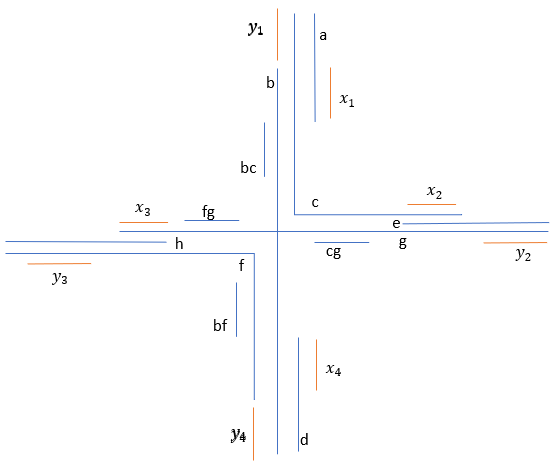
\includegraphics[width=12cm]{./img/representacaoFalsePieGadgetClausula.png}\label{fig:falsePie}}
% \qquad
% \subfloat[Representação de Torta Verdadeira]{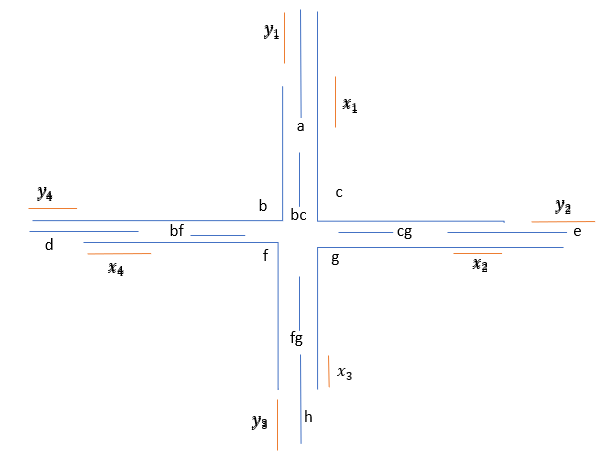
\includegraphics[width=12cm]{./img/representacaoTruePieGadgetClausula.png}\label{fig:truePie}}
% \qquad
\subfloat[][Representação de quadro (frame)]{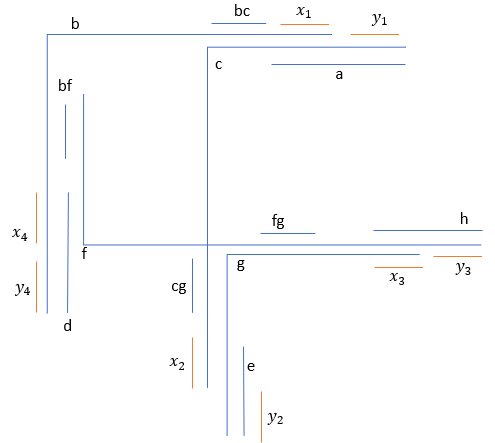
\includegraphics[width=12cm]{./img/representacaoFrameGadgetClausula.png}\label{fig:frame}}
\caption{Representação estrutural $B_{1H}(G_{C})$, como quadro.}
\end{figure}  
  